%!TEX root = paper.tex
\subsection{Data}

\indent{\indent The dataset is a part of the database that has been recorded at Aarhus University Flakkebjerg Research station in a collaboration between the University of Southern Denmark and Aarhus University. Images are available to researches at \url{https://vision.eng.au.dk/plant-seedlings-dataset/}. The specific of the dataset is that recorded plants are in different growth stages since detecting weed in its early stage is the thing makes the task problematic. }

\indent{The dataset contains 960 unique plant images of 12 species. The sizes of plant classes are not balanced among themselves - they range from 221 to 654 labeled samples for each class. Original images are cropped by plant boundaries, but their resolutions vary from 50x50px to 2000x2000px. Also, images have a different background - some of them on the ground, other on the marked paper.}
\begin{figure}[h]
    \centering
    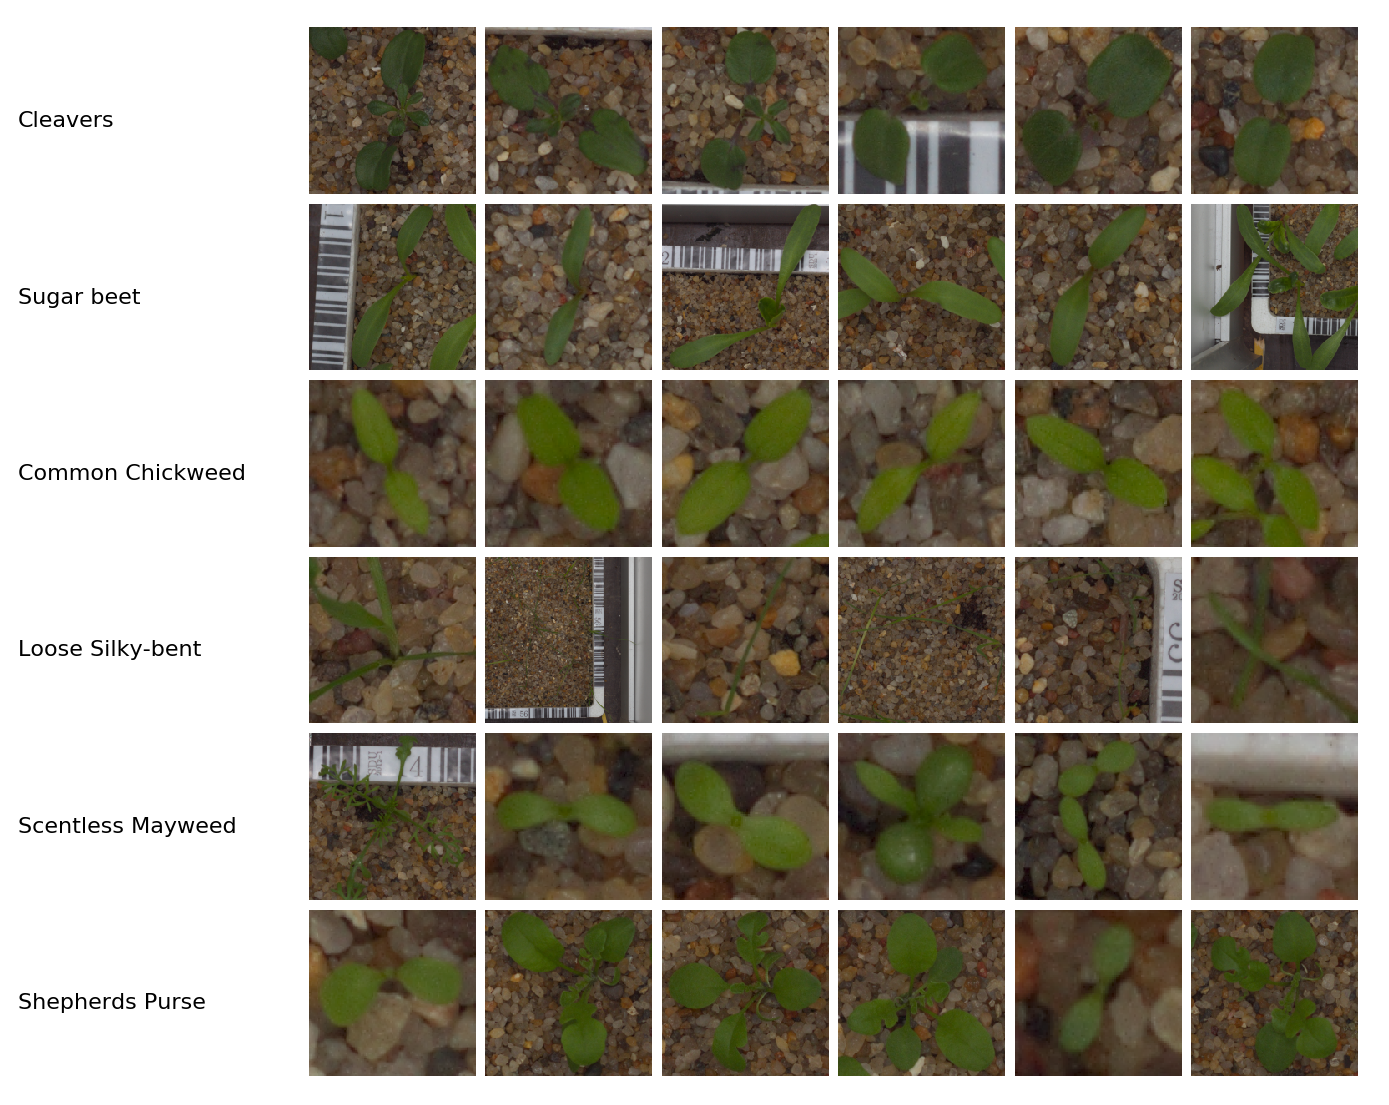
\includegraphics[height=8.5cm, width=10.5cm]{first_view_grid_smaller_1}
    \caption{Data overview}
    \label{fig:1}
\end{figure}

\subsection{Data preprocessing}
\indent{\indent \textbf{Resolution reducing}}

\indent{We reduce the resolution of all images to the same resolution 200x200px using bilinear interpolation. The main idea of bilinear interpolation that the new image pixel is the weighted sum of neighboring pixels of the original image. It helps to decrease computational complexity and build normalized features.}

\textbf{Segmentation}

\indent{The objects of our study are plants, and they are painted green. Therefore, we can create a mask that filters the range of green channel and ignores the other pixels. For these purposes, the HSV (Hue Saturation Value) color model is a suitable representation. In the BGR format, the value of each component depends on the amount of light hitting the object. HSV allows us to distinguish between image color and brightness. Hue, saturation, and value let us set the lower and upper borders of the shades of a certain color, in this case –– green. Then we merely mark the pixels in the green range and get a color mask (Fig. \ref{fig_f_ seg_step_2}). Now we apply the operation of logical multiplication to the original image, assign the value of the background pixels to a black color value, and get a segmented plant.}

\threeimage{seg_step_1}{seg_step_2}{seg_step_3}{Source image}{Mask}{Segmented image}

\textbf{Noise removal}

\indent{Segmentation does not always work well (Fig. \ref{fig_f_ seg_step_3}). Small areas of the background may fall into the range of green values which distorts the binary mask (Fig. \ref{fig:seg_no_morph_1})}.

\begin{figure}[h]
	\centering
    \subfigure[Before morphological closure]{
		{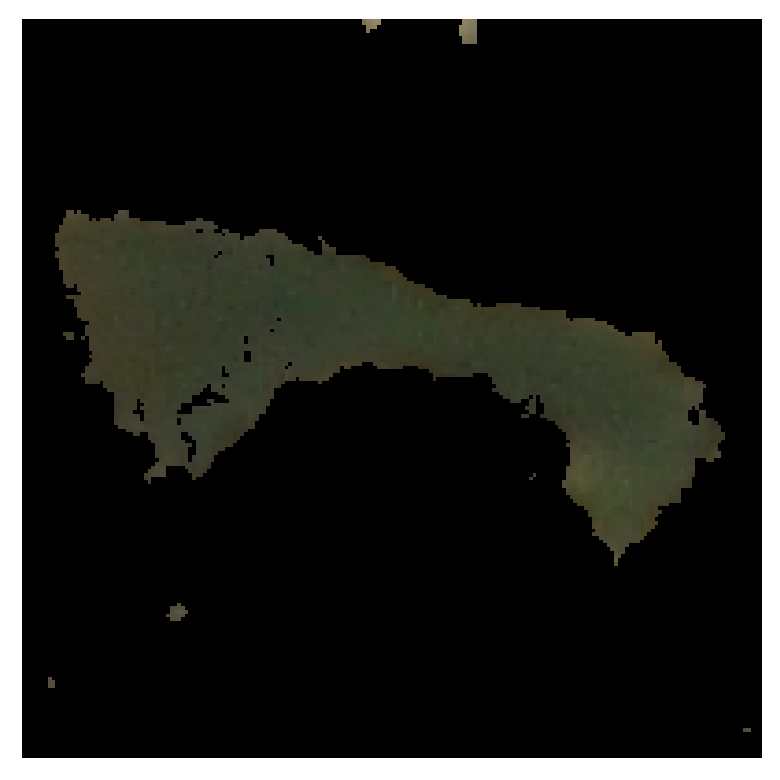
\includegraphics[width=5cm, height=5cm]{seg_no_morph_1}
		\label{fig:seg_no_morph_1}}
	}
    \qquad
    \subfigure[After morphological closure]{
		{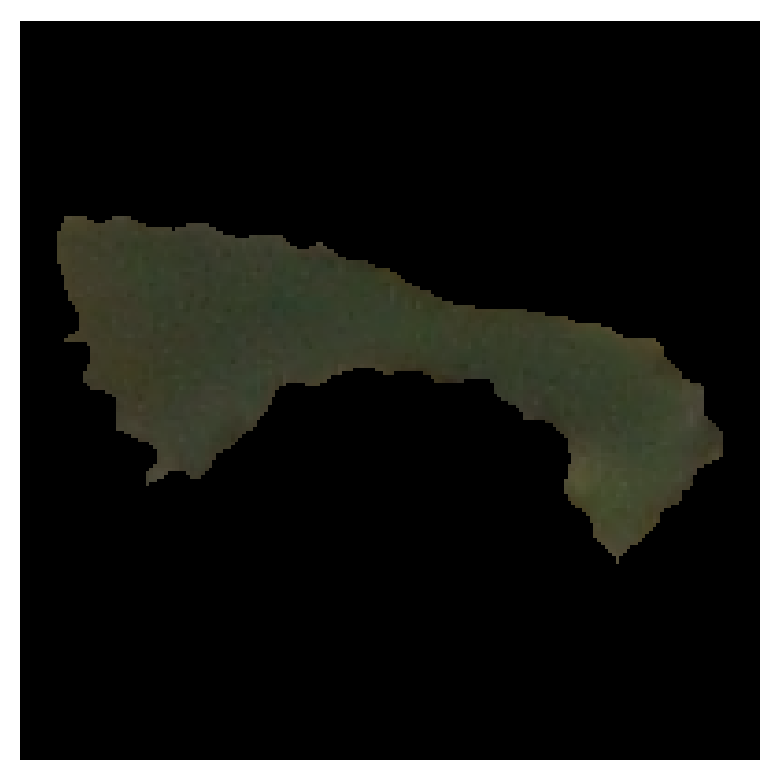
\includegraphics[width=5cm, height=5cm]{seg_morph_1}
		\label{seg_morph_1}}
	}
    \caption{Segmentation improvement example}%
    \label{fig:seg_improve}
\end{figure}

\indent{Such drawbacks can be eliminated with the morphological operations –– nonlinear transformations associated with the shape and structure of image. The morphology is used to study the interaction of an image with a specific structural element –– the kernel. The kernel iterates over the entire image and compares with the neighborhood of the pixels after which we apply morphological operations \cite{friel2000imanalysis}.}

\indent{To improve segmentation, we use the operation of morphological closure –– a combination of dilatation and erosion operations.}

\indent{Then we apply the morphological closure operation to the image (Fig. \ref{fig:seg_no_closure_good_1}) by selecting an elliptical core of 6x6px size and delete the remaining objects with an area of less than 160px. The plant on the image (Fig. \ref{fig:seg_with_closure_bad_1}) has no cavities, and the background is cleared of non-plant elements. But morphological closure does not always improve the segmentation result. Estimate the result of working on an image of the class Loose silky-bent. It is noticeable (Fig. \ref{fig:seg_degradation}) that the cavities corresponding to the background were restored, which does not correspond to the desired result. We restrict ourselves to the removal of objects whose contours limit a small area.}

\begin{figure}[h]
	\centering
    \subfigure[Before morphological closure]{
		{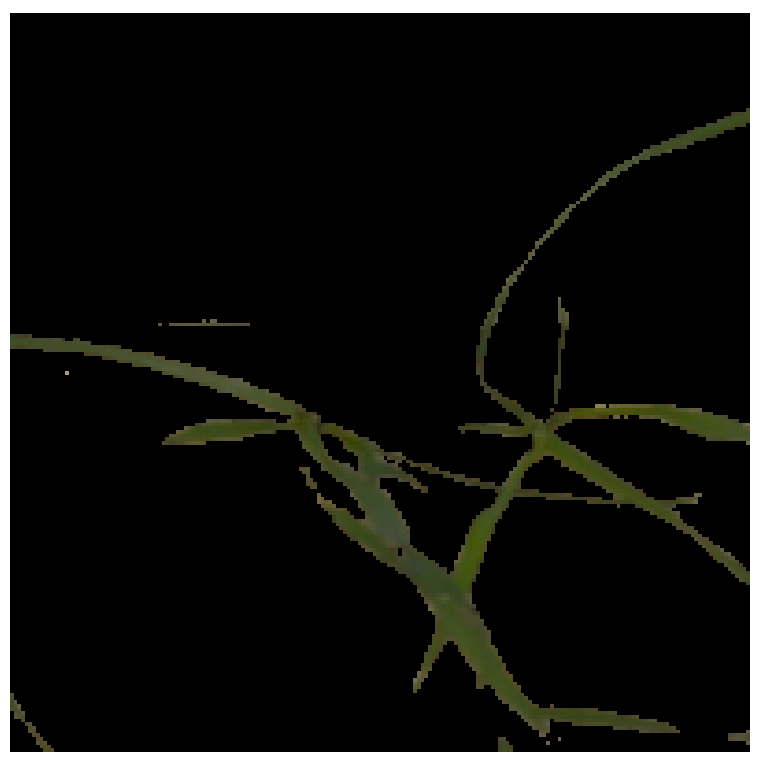
\includegraphics[width=5cm, height=5cm]{seg_no_closure_good_1}
		\label{fig:seg_no_closure_good_1}}
	}
    \qquad
    \subfigure[After morphological closure]{
		{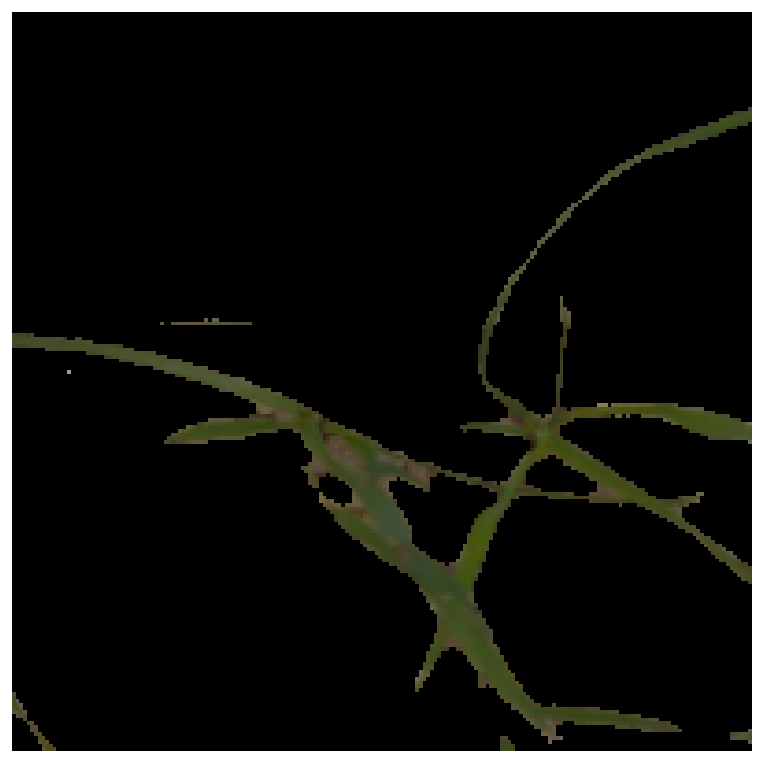
\includegraphics[width=5cm, height=5cm]{seg_with_closure_bad_1}
		\label{fig:seg_with_closure_bad_1}}
	}
    \caption{Segmentation degradation example}%
    \label{fig:seg_degradation}
\end{figure}
